\documentclass[11pt]{article}

\usepackage[margin=1in]{geometry}
\usepackage{graphicx}
\usepackage{subcaption}
\usepackage{amsmath}
\usepackage{amssymb}
\usepackage{float}

\title{RL Lab 4 - MC Control, Q-Learning and Expected Sarsa}
\author{Adonis Jamal}
\date{}

\begin{document}
\maketitle

\section{MC control on blackjack}
\subsection{Interpret the graph}


\begin{figure}[H]
    \centering
    \begin{subfigure}{0.48\textwidth}
        \centering
        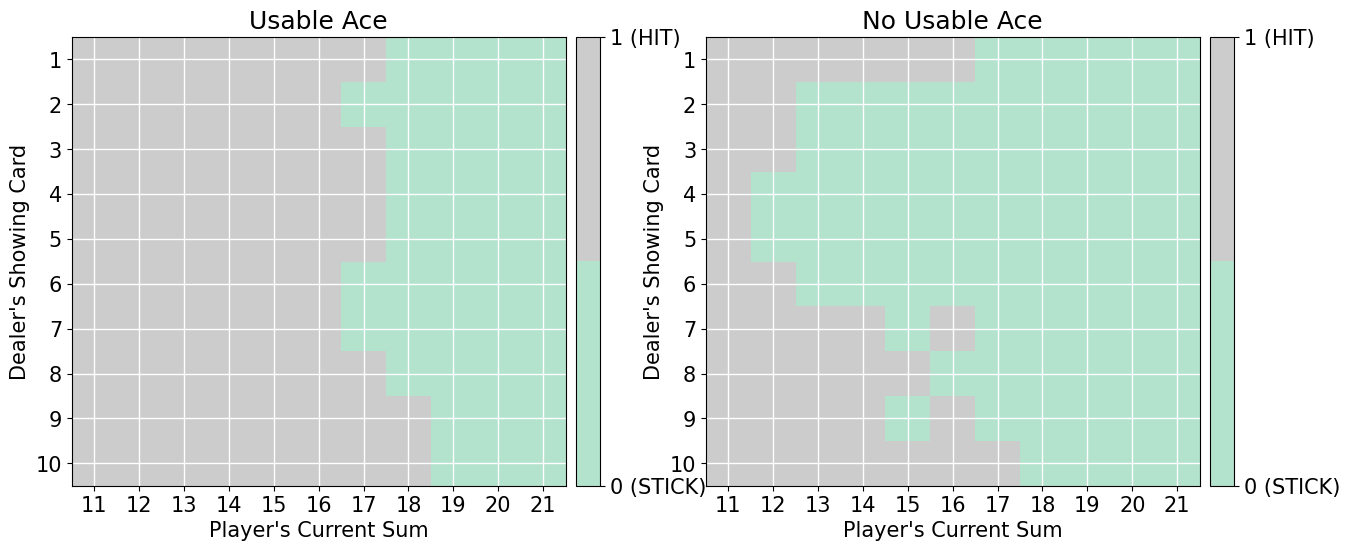
\includegraphics[width=\textwidth]{figures/1 MC Control on BlackJack.png}
        \caption{Optimal policy learned by MC Control. Left: with usable ace (hit below 19). Right: without usable ace (dealer-dependent).}
    \end{subfigure}
    \hfill
    \begin{subfigure}{0.48\textwidth}
        \centering
        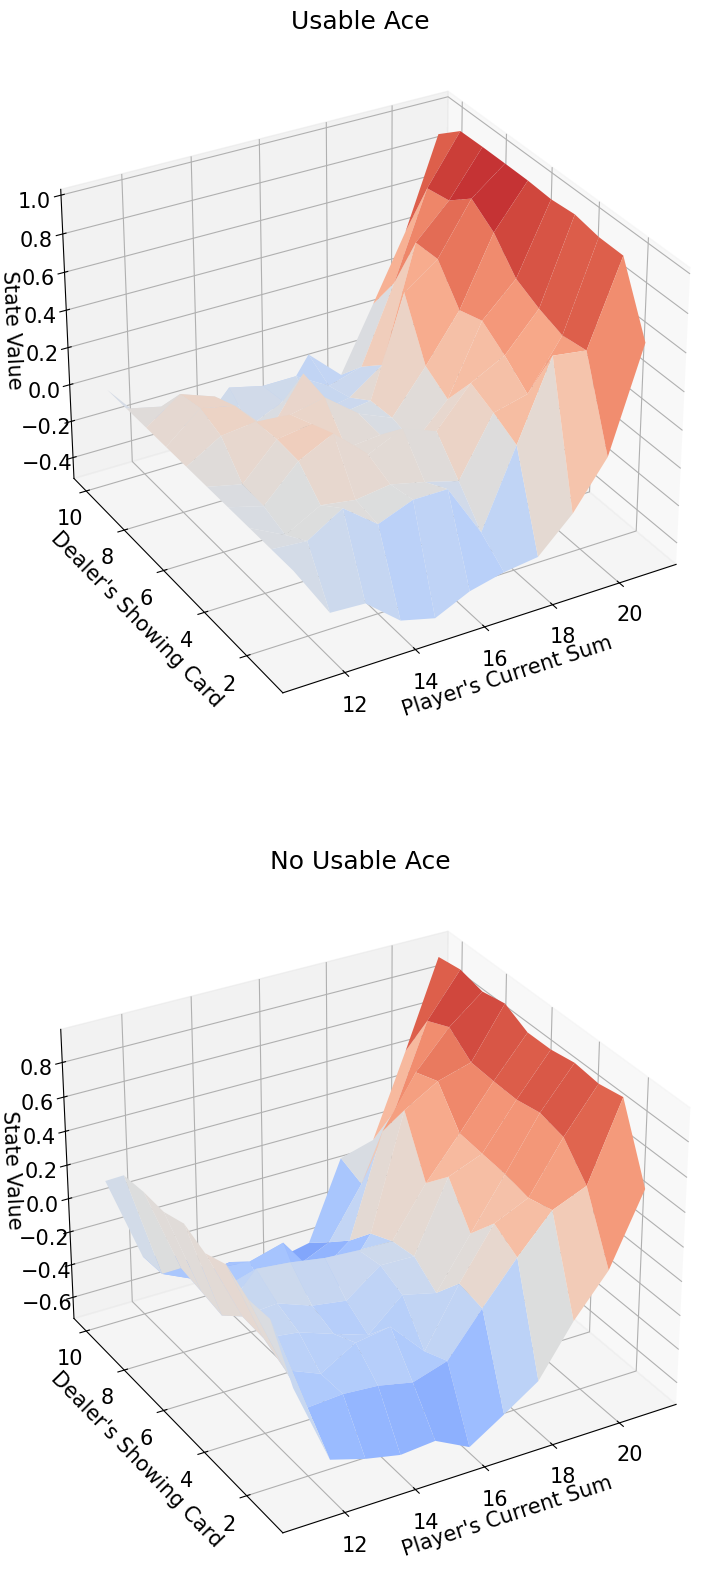
\includegraphics[width=0.4\textwidth]{figures/1 state value.png}
        \caption{State-value function for Blackjack. Top: with usable ace (higher values). Bottom: without usable ace (values depend on player sum and dealer card).}
    \end{subfigure}
\end{figure}

These graphs show the optimal policy and state-value function learned by MC Control. The policy displays two distinct strategies: with a usable ace, the agent aggressively hits below 17 due to the safety buffer a usable ace provides. Without a usable ace, the strategy becomes dealer-dependent hitting when the dealer shows strong cards (7+), but sticking at 12+ against weak dealer cards (2-6), recognizing the dealer's bust probability. 

The 3D value function surface shows that states with a usable ace are inherently more valuable, with peaks at player sums of 19-21. Without a usable ace, state values depend critically on both the player's hand strength and the dealer's exposed card. Both policies align with basic Blackjack strategy, demonstrating that the agent discovered optimal decision factors: player hand strength, dealer visibility, and ace flexibility. Some noise appears due to insufficient visitation of certain state-action pairs despite 500,000 episodes.


\section{Solving the Cliff World}
\subsection{Interpret the plot}
\begin{figure}[H]
    \centering
    \begin{subfigure}{0.48\textwidth}
        \centering
        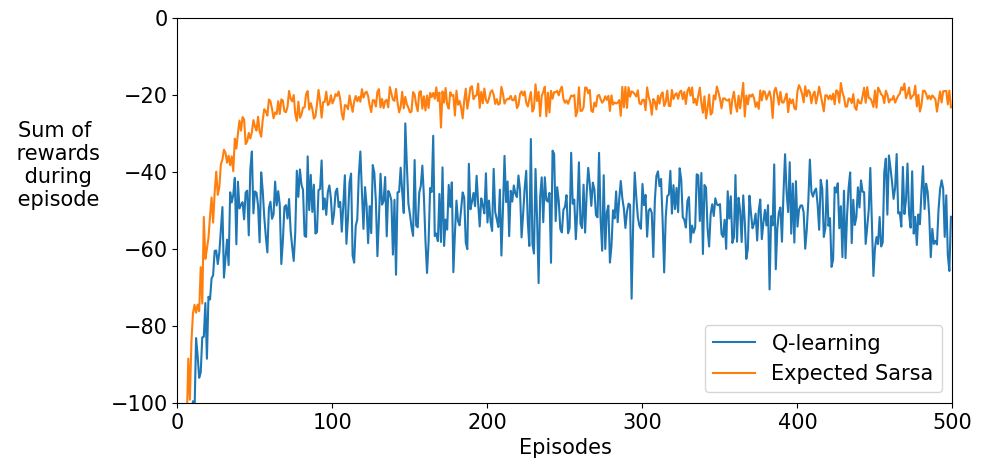
\includegraphics[width=\textwidth]{figures/2 cliff world rewards.png}
        \caption{Sum of rewards per episode over 500 episodes trained on Cliff World. Expected Sarsa converges to higher (less negative) rewards than Q-learning.}
    \end{subfigure}
    \hfill
    \begin{subfigure}{0.48\textwidth}
        \centering
        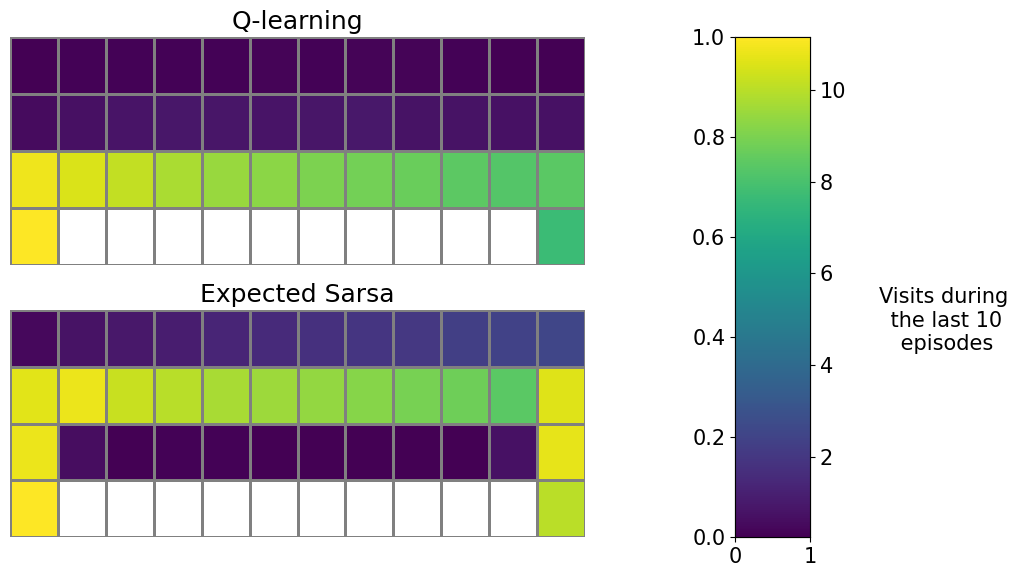
\includegraphics[width=\textwidth]{figures/2 cliff world states.png}
        \caption{State visitation heatmaps during the last 10 episodes. Expected Sarsa takes a safer path away from the cliff, while Q-learning takes a risky path close to the cliff edge.}
        \label{fig:cliff_world_results}
    \end{subfigure}
\end{figure}

Figure~\ref{fig:cliff_world_results} shows the number of timesteps that each agent spent in each state over the last 10 episodes in the Cliff World environment.

From the plot, we can see that the Q-learning agent spends more time in the states closer to the cliff, which indicates that it is exploring those states more. This is likely because Q-learning is an off-policy algorithm that learns the optimal policy regardless of the agent's actions, learning the shortest path to reach the goal at the expense of ignoring the risk of falling off the cliff.

On the other hand, the Expected Sarsa agent avoids the states near the cliff, which suggests that it is more cautious and prioritizes safety over reaching the goal quickly. Expected Sarsa is an on-policy algorithm that learns the value of the policy being followed, which may lead to more conservative behavior as it takes into account the risk associated with certain actions.

\begin{figure}[H]
    \centering
    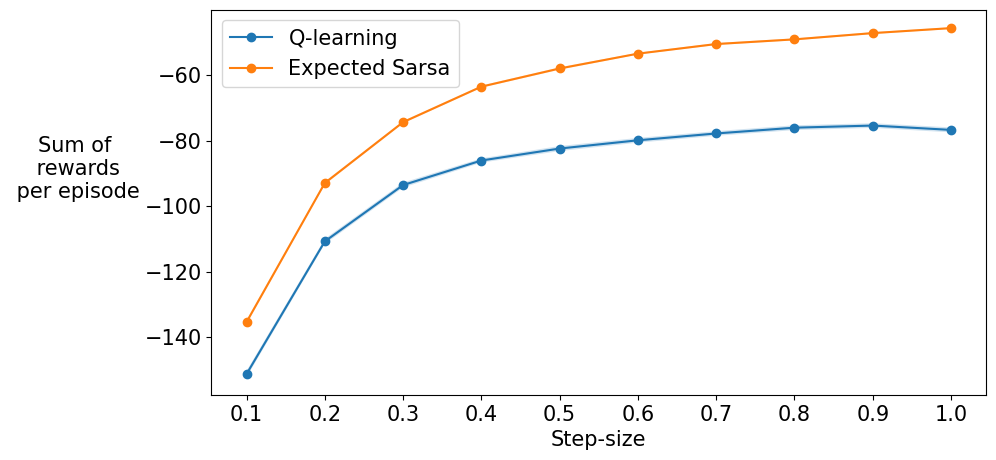
\includegraphics[width=0.8\textwidth]{figures/2 cliff world step size.png}
    \caption{Sum of rewards per episode for different step sizes. Expected Sarsa consistently outperforms Q-learning across all step sizes.}
\end{figure}

The graph above shows the average sum of rewards per episode for both the Q-learning and Expected Sarsa agents across different step-sizes.

Expected Sarsa consistently outperforms Q-learning across all step-sizes, as indicated by the higher average rewards. This suggests that Expected Sarsa's on-policy learning approach allows it to learn a more effective policy in the Cliff World environment compared to Q-learning's off-policy approach.

The $\epsilon$-greedy exploration strategy used by Q-learning leads to lower rewards, especially at higher step-sizes, as it causes the agent to take the optimal risky path, taking riskier actions that may lead to falling off the cliff, as shown in the state visitation plot. In contrast, Expected Sarsa's more cautious approach results in higher rewards, as it avoids the cliff and learns a safer policy. While the policy learned by Expected Sarsa is more conservative and not the optimal path to the goal, it yields higher rewards due to avoiding the negative consequences of falling off the cliff.

\end{document}
